
\section{Introducere}

În acest capitol voi vorbi de următorul element principal care oferă încredere conținutului distribuit de aplicația TrustNews și anume despre Zero Knowledge Proofs (\textit{ZKPs}). Voi aborda elementele criptografice de bază și etapele ce trebuie desfășurate pentru a putea genera și folosi o structură de dovedire.\\

\section{Concepte criptografice}

Conceptul de la care se pornește este criptografia bazată pe curbe eliptice. O curbă eliptică este reprezentarea în plan a unei funcții non-singulare definită fie de ecuația $C: y^2 = x^3 + ax +b$, fie de ecuația $C: by^2 = x^3 + ax^2 +x$. Câmpul de valori este grupul finit $\mathbb{F}_p$ unde p este un număr prim suficient de mare \cite{ZKS_Crypto_Basic}. Calculele se vor efectua modular având ca modul numărul p. De exemplu curba eliptică folosită pentru generarea perechilor de chei asimetrice din cadrul BigchainDB este Curve25519 \cite{ZKS_Curve25519} care are ecuația $y^2 = x^3 + 48666x^2 + x$ cu $p = 2^{255} - 19$.\\

Criptografia în acest context se bazează pe ECDLP acronim ce provine de la \textit{Elliptic Curve Discret Logarithm Problem} (Problema algoritmului discret pe curbe eliptice). ECDLP presupune existența perechilor de puncte $\mathcal{P}$ și $\mathcal{Q}$ pe curba C cu valori în câmpul finit $\mathbb{F}_p$ și a unui număr întreg k astfel încât $k\mathcal{P} = \mathcal{Q}$. Dacă $\mathcal{P}$ și k sunt cunoscute atunci găsirea punctului $\mathcal{Q}$ se poate realiza eficient, dar dacă se cunosc doar punctele $\mathcal{P}$ și $\mathcal{Q}$ problema găsirii numărului k este foarte dificilă.\\

\clearpage

O curbă eliptică în plan realizată peste numerele reale va arăta întotdeauna continuă și va fi simetrică față de axa Ox. În momentul în care restrângem la câmpul finit $\mathbb{F}_p$ graficul devine o colecție de puncte sau mai exact o colecție de perechi de puncte, elementele din perechi vor fi simetrice față de axa imaginară dată de $y = p/2$.

\begin{figure}[H]
    \centering
    \subfloat[In $\mathbb{R}$]{{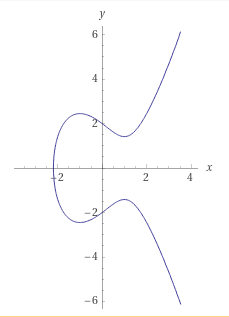
\includegraphics[scale=0.7]{Images/EC_Example_R.png}}}
    \qquad
    \subfloat[In $\mathbb{F}_{17}$]{{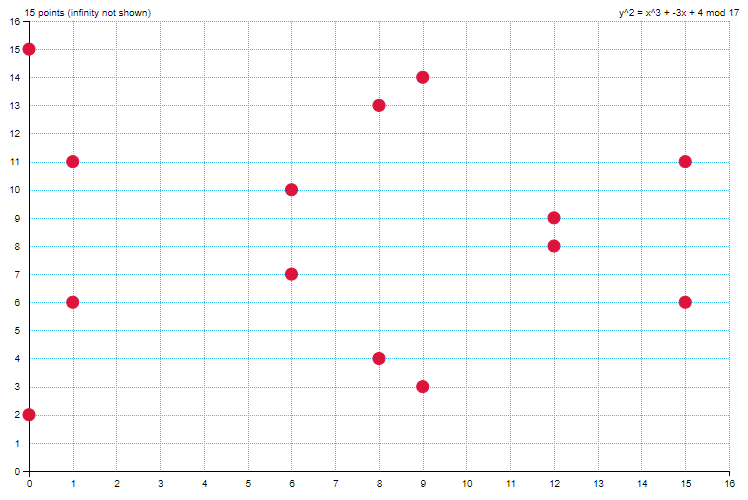
\includegraphics[scale=0.4]{Images/EC_Example_F17.png}}}
    \caption{Curba eliptică $C: y^2 = x^3 - 3x + 4$; Grafice realizate cu \cite{WolframAlpha} și \cite{Graui}}
\end{figure}

Înainte de a defini operațiile pe care le putem face trebuie să definim elementul neutru numit și punctul la infinit care satisface relațiile $\mathcal{P} + \mathcal{O} = \mathcal{P}$ și $\mathcal{P} + (-\mathcal{P}) = \mathcal{O}$ pentru orice $\mathcal{P}$.\\

Negația unui punct $\mathcal{P}(x_p,y_p)$ se definește ca simetricul său față de axa imaginară $y = p/2$ $( -P = (x_p, -y_p) )$. Adunarea dintre două puncte $\mathcal{P}$ și $\mathcal{Q}$ se definește grafic ca negația punctului de intersecție dintre curbă și dreapta dată de cele două puncte $(P(x_p, y_p) + Q(x_q, y_q) = R(x_r, y_r) \Rightarrow -R)$. În situația în care $\mathcal{P}$ = $\mathcal{Q}$ adunarea se numește dublare iar dreapta dată de punct este tangenta. Înmulțirea cu un scalar k poate fi acum definită ca suma repetată a aceluiași punct.\\

Peste punctele de pe curbe eliptice se pot defini perechi date de funcții de evaluare biliniare notate $e: \mathbb{G}_1 \times \mathbb{G}_2 \rightarrow \mathbb{G}_T$. Mulțimile $\mathbb{G}_1$ și $\mathbb{G}_2$ formează cu operația de adunare grupuri comutative iar mulțimea $\mathbb{G}_T$ formează grup comutativ cu operația de înmulțire. Aceste funcții trebuie să respecte biliniaritatea și non-degenerarea date de condițiile:
\begin{itemize}
    \item $e(\mathcal{P},\mathcal{Q} + \mathcal{R}) = e(\mathcal{P},\mathcal{Q}) \cdot e(\mathcal{P},\mathcal{R}), \quad \forall \mathcal{P} \in \mathbb{G}_1, \forall \mathcal{Q},\mathcal{R} \in \mathbb{G}_2$
    \item $e(\mathcal{P}+\mathcal{Q},\mathcal{R}) = e(\mathcal{P},\mathcal{R}) \cdot e(\mathcal{Q},\mathcal{R}), \quad \forall \mathcal{P},\mathcal{Q} \in \mathbb{G}_1, \forall \mathcal{R} \in \mathbb{G}_2$
    \item $\forall \mathcal{P} \in \mathbb{G}_1, \mathcal{P} \neq 0,\quad \exists \mathcal{Q} \in \mathbb{G}_2: e(\mathcal{P},\mathcal{Q}) \neq 1$
    \item $\forall \mathcal{Q} \in \mathbb{G}_2, \mathcal{Q} \neq 0,\quad \exists \mathcal{P} \in \mathbb{G}_1: e(\mathcal{P},\mathcal{Q}) \neq 1$
\end{itemize}

\clearpage

Alte procedee utile în ZKPs sunt schemele de comitere și criptarea homomorfică.\\

Schema de comitere presupune stabilirea unei informații și păstrarea ei sub formă criptată până la decizia celui care o criptează de a o face publică. Valoarea ascunsă poate fi și publicată având siguranța că nu se pot extrage informații din aceasta \cite{ZKS_Crypto_Basic}. \\

Criptarea homomorfică este cea care ne permite să folosim valoarea criptată mai departe în operații, urmând ca decriptarea valorii finale va fi egală cu procesarea valorii inițiale. Pentru ca o funcție HE(x) să poată da acest comportament trebuie să satisfacă următoarele criterii \cite{ZKS_Crypto_Basic}:
\begin{itemize}
    \item Este ușor de calculat HE(x) pornind de la x, dar având HE(x) este foarte dificilă găsirea lui x.
    \item Două valori diferite x și y vor rezulta în două valori HE(x) și HE(y) diferite
    \item Liniaritatea trebuie păstrată: $HE(\alpha x + \beta y) = \alpha HE(x) + \beta HE(y)$
\end{itemize}

Pentru a răspunde tuturor cerințelor se apelează la o formă de criptare $HE(x) = g^x$. Aritmetica se realizează peste $\mathbb{Z}_p$, unde p este un număr prim mare. Valoarea g este aleasă ca generatorul grupului ciclic $\mathbb{Z}^*_p$, care ne poate da toate valorile din grup ridicând-o la puteri diferite. Primul criteriu este satisfacut de problema algoritmului discret, $HE(x) = g^x (mod \ p)$ va fi ușor de calculat dar aflarea lui x cunoscând HE(x) este grea. Criteriul liniarității este satisfacut, $HE(x + y) = g^{x+y} = g^x \cdot g^y = HE(x) \cdot HE(y)$ unde $x \ne y \rightarrow HE(x) \ne HE(y)$.\\

Alte elemente țin de problema criptării folosind polinoame. Acestea vom vedea că stau la baza programelor aritmetice care pentru a-și demonstra corectitudinea trebuie să satisfacă o relație de forma $t(x)h(x) = l(x)r(x) - o(x)$, unde t,h,l,r,o sunt polinoame \cite{ZKS_Crypto_Basic2}.\\

\clearpage

\section{Zero-Knowledge Proofs (ZKPs)}

Un mecanism de tip Zero-Knowledge Proof este un protocol criptografic între două părți comunicante în care un doveditor convinge un verificator că o informație este adevărată sau că se cunoaște o anumită informație fără a o expune direct verificatorului \cite{ZKS_Crypto_Basic}.\\

Pentru ca interacțiunea dintre doveditor și verificator să se realizeze pe baza unui ZKP corect, acesta trebuie să respecte anumite proprietăți.
\begin{itemize}
    \item \textbf{Completness}. Proprietatea asigură că dacă ambii participanți sunt onești atunci se respectă convenția protocolului, un doveditor vrea să demonstreze că știe o informație adevărată iar un verificator se va convinge că informația este întradevăr cum susține doveditorul că este.
    \item \textbf{Soundness}. Dacă doveditorul încearcă să păcălească verificatorul atunci acesta își poate da seama cu probabilitate mare și poate să refuze dovada primită.
    \item \textbf{Zero-Knowledgeness}. Caracterul Zero-Knowlegde se referă la incapacitatea verificatorului de a afla informația propriu-zisă pe care încearcă doveditorul să o demonstreze. El poate afla doar valoarea de adevăr pentru ceea ce susține doveditorul.
\end{itemize}

În sine un protocol ZKP standard este un proces interactiv în care cei doi membri pot transmite mesaje în mai multe etape consecutive și independente până când decid amândoi că ceea ce sustin este corect. Un celebru exemplu este peștera lui Ali Baba \cite{ZKS_AliBaba}. Problema implică o peștera în formă circulară cu o singură intrare și cu o poartă magică la mijlocul formei circulare. Alice vrea să îl convingă pe Bob că știe parola pentru a deschide ușa fără să îi spună direct. Pentru a se convinge Bob alege să rămână în afară peșterii, în timp ce Alice alege să meargă pe oricare din cele două direcții posibile până ajunge la ușa. Apoi Bob intră în peștera până la bifurcatie și o roagă pe Alice să vină pe un drum ales de el. Dacă drumul ales de Bob este de partea opusă ușii, Alice va trebui să folosească parola și să iasă pe partea cerută demonstrându-i lui Bob că poate face acest lucru. Procesul se poate repeta de oricâte ori până când Bob este convins că Alice știe cu adevărat parola și nu doar ghicește. \\

\begin{figure}[H]
    \centering
    \subfloat[]{{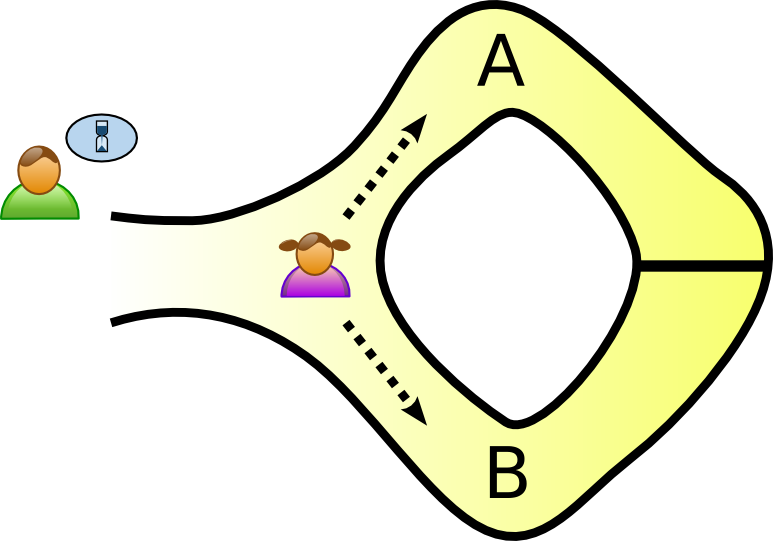
\includegraphics[scale=0.15]{Images/ZKS_AliBaba1.png}}}
    \qquad
    \subfloat[]{{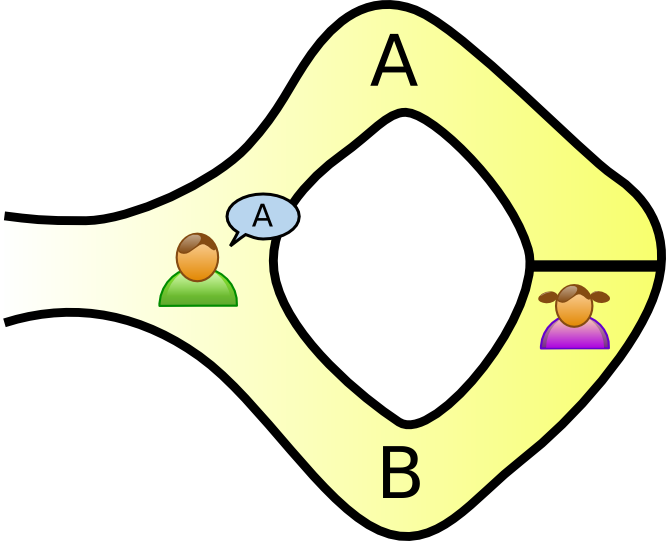
\includegraphics[scale=0.15]{Images/ZKS_AliBaba2.png}}}
    \qquad
    \subfloat[]{{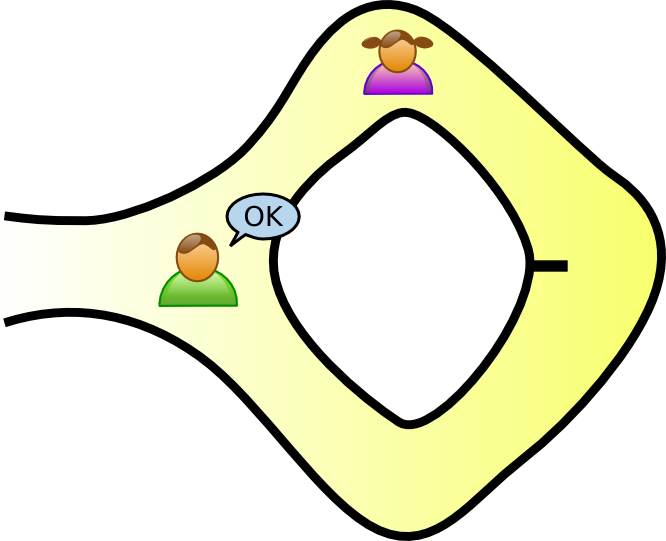
\includegraphics[scale=0.15]{Images/ZKS_AliBaba3.png}}}
    \caption{Problema peșterii lui Ali Baba - sursă \cite{ZKS_Wikipedia}}
\end{figure}

\section{zkSNARKs}

Abrevierea zkSNARKs provine de la Succinct Non-interactive Arguments of Knowledge și este construit peste conceptul prezentat anterior moștenind proprietățile acestuia \cite{ZKS_Crypto_Basic2}.\\

Caracterul succint vine de la faptul că mesajele transmise între cele două părți comunicante au dimensiuni foarte mici. Practic computatia realizată pentru crearea unei dovezi ne permite ca în final să avem structuri mici care se pot verifica foarte ușor \cite{ZKS_Crypto_Basic2}. \\

Se elimină nevoia de interacțiune între cei doi, va exista o etapă de preprocesare după care un singur mesaj va fi suficient pentru a trimite dovada. Verificarea va putea fi efectuată de oricine fără a fi nevoie de interacțiune în plus și ajută în principal atunci când este folosită în cadrul blockchain unde orice nod ar putea verifica o dovadă asociată oricărei tranzacții \cite{ZKS_Crypto_Basic2}.\\

Argumentele fac referire la proprietatea de soundness și implică faptul că un verificator poate avea încredere doar într-un doveditor cu resurse de procesare limitate. Un doveditor malițios cu suficient de multă putere de procesare poate crea dovezi ce au la bază informații false și care pentru verificator par corecte \cite{ZKS_Crypto_Basic2}.\\

Caracterul de cunoaștere este adresat doveditorului ce trebuie să cunoască setul de informații numit și witness pentru a putea construi o dovadă pe baza lui. Totodată verificatorul nu află nimic despre valorile acestor informații.\\

Dovezile de tip zkSNARKs se pretează, din câte se cunoaște până acum, problemelor din clasa NP. Această clasă de probleme este o generalizare a clasei P ce curpinde programe rezolvabile într-o complexitate polinomiala \cite{ZKS_Crypto_Basic2}. Clasa de probleme NP se poate descrie ca mulțimea problemelor L care conțin la rândul lor un program V de complexitate polinomială și care este folosit pentru a verifica o informație cunoscând de asemenea un witness de dimensiune polinomială. Putem spune și că programul L având ca dată de intrare x se termină și întoarce o valoare de adevăr pozitivă dacă există un witness w astfel încât V(x,w) să întoarcă valoarea de adevăr pozitivă. \\

Un exemplu de problema NP este cea a verificării satisfiabilității unei formule SAT(f). Verificarea se poate realiza pentru orice funcție în timp polinomial dar doar cu ajutorul unui witness care în cazul acesta va cuprinde valorile de adevăr asociate fiecărei variabile astfel încât valoarea de adevăr a întregii formule să fie 1. De la acest exemplu se poate defini și proprietatea asociată oricărui program NP și care spune că un program L(x) poate fi echivalat cu SAT(f(x)). Verificarea unei tranzacții în blockchain poate fi un exemplu, problema se reduce la satisfacerea unei formule create pe baza criteriilor de construcție a unei tranzacții, witness-ul aici va consta din valori corecte incluse în tranzacție \cite{ZKS_Crypto_Basic}.\\

\section{Quadratic Programs}

Un Quadratic Span Program (\textit{QSP}) constă într-un set de polinoame iar problema pe care o rezolvă este găsirea unei combinații liniare astfel încât produsul rezultat să fie un multiplu al unui alt polinom țintă \cite{ZKS_Crypto_Basic2}. Mai mult decât atât coeficientii din polinoame vor fi dictați de input-urile programul și de witness.\\

Un program QSP peste un spațiu finit $\mathbb{F}$ cu input de lungime $n$ conține o serie de polinoame $v_0,...v_m$, o serie de polinoame $w_0,...,w_m$, un polinom țintă t și o funcție injectivă $f:\{(i,j) \ | \ 1 \leq i \leq n, \  j \in \{0,1\}\}\rightarrow\{1,...,m\}$. Validarea unui input $u$ se face doar dacă există coeficienții $a_1,...,a_m,\ b_1,...,b_m$ astfel încât polinomul țintă $t$ să dividă $(v_0 + a_1v_1 + ... + a_mv_m)(w_0 + b_1w_1 + ... + b_mw_m) = v_aw_b$ cu $a_k,b_k = 1$ dacă există perechea de forma $(i,u[i])$ pentru care $f(i,u[i])\ =\ k$, u[i] = Valoarea bit-ul de pe poziția i și $a_k,b_k = 0$ în rest.\\

Procesul prin care doveditorul arată că știe o informație se transformă în dovedirea că știe o soluție al programului QSP. Cu alte cuvinte dovedește ca input-ul $u$ știut de el generează seriile de coeficienți $a_k$ și $b_k$ cu care poate calcula polinomul $h$ astfel încat $th-v_aw_b=0$.\\

Acțiunea verificatorului va fi validarea ecuației menționate anterior. Pentru a reduce complexitatea procesului de validare se pot alege valoari $s_i$, se pot evalua polinoamele obținând $t(s_i),v_a(s_i),w_b(s_i)$ și se pot verifica ecuațiile $t(s_i)h(s_i)\ =\ v_a(s_i)w_b(s_i)$ \cite{ZKS_Crypto_Basic2}.\\

Superioare programelor descrise anterior sunt Quadratic Arithmetic Program (QAP) care merg pe un drum similar însă pot valida construcții aritmetice și se folosesc de 3 polinoame în locul celor 2 ($v_a$ și $w_b$) de la QSP \cite{ZKS_Crypto_Basic}.\\

Construcția acestor tipuri de programe se bazează pe circuite aritmetice. Aceste circuite nu sunt altceva decât grafuri orientate ce pornesc de la valori de input, care se unesc prin fire de porți reprezentând operațiile aritmetice efectuate \cite{ZKS_Crypto_Basic3}. De exemplu, ceea ce formal se poate scrie ca $C: \mathbb{F}^2 \times \mathbb{F}^2 \rightarrow \mathbb{F}, C(a_1,a_2,a_3,a_4) = (a_1 + a_2) * a_3 * (a_3 - a_4)$ se poate reprezenta grafic în imaginea urmatoare.\\

\begin{figure}[H]
\centering
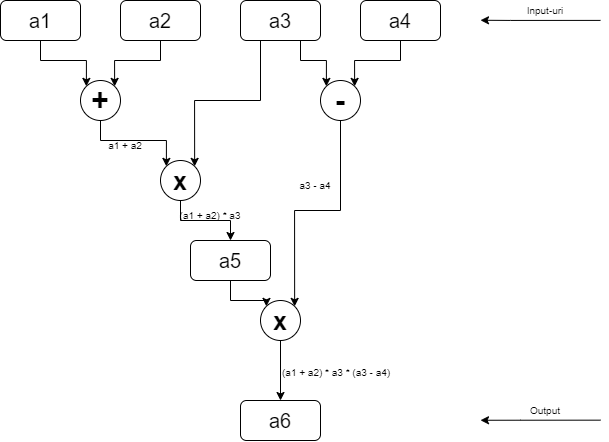
\includegraphics[scale=0.6]{Images/ZKS_QAP_Example.png}
\caption{Exemplu circuit aritmetic - Grafic realizat cu \cite{Diagrams}}
\end{figure}

Se definește mulțimea punctelor țintă M conținând indecși pentru fiecare poartă folosită pentru operația de înmulțire și mulțimea W ce conține fire folosite pentru input-urile programului și etichete output-urilor porților înmulțire \cite{ZKS_Crypto_Basic4}. Pe baza mulțimii M se definește polinomul țintă $T(x)$ de grad $d$ ca fiind $\prod_{g\in\mathbb{M}} (x - r_g)$ unde $r_i$ sunt rădăcini diferite. Pentru exemplul de sus $T(x) = (x-r_5)(x-r_6)$.\\

Pe lângă polinomul țintă se definesc 3 mulțimi de polinoame \cite{ZKS_Crypto_Basic3}:
\begin{itemize}
    \item Polinoamele de la stânga. $L_i(r_g) = c_{g,L,i},\ i \in I_{g,L}$ și $L_i(r_g) = 0$ în rest
    \item Polinoamele de la dreapta. $R_i(r_g) = c_{g,R,i},\ i \in I_{g,R}$ și $R_i(r_g) = 0$ în rest
    \item Polinoamele de output. $O_i(r_g) = 1,\ dacă\ i = g$ și $O_i(r_g) = 0$ în rest
\end{itemize}

$I_{g,L}$ și $I_{g,R}$ sunt submulțimi ale lui W și reprezintă etichetele sau firele ce intră în poarta $g$ venind din stânga, respectiv dreapta, și care nu au mai fost folosite în alte porți multiplicative înaintea lui $g$.
$c_{g,L,i}$ și $c_{g,R,i}$ sunt coeficienții cu care eticheta $i$ intră în poarta $g$ venind din stânga, respectiv dreapta.
$L_0(r_g)$ respectiv $R_0(r_g)$ vor fi valorile constantelor ce intră în porțile $g$. 
Se vor calcula valorile pentru fiecare poartă multiplicativă.

Valorile asociate evaluărilor polinoamelor pentru exemplul de sus sunt
\begin{multicols}{3}
$L_0(r_5) = 0$ \\
$L_0(r_6) = 0$ \\
$L_1(r_5) = 1$ \\
$L_1(r_6) = 0$ \\
$L_2(r_5) = 1$ \\
$L_2(r_6) = 0$ \\
$L_3(r_5) = 0$ \\
$L_3(r_6) = 0$ \\
$L_4(r_5) = 0$ \\
$L_4(r_6) = 0$ \\
$L_5(r_5) = 0$ \\
$L_5(r_6) = 1$ \\
$L_6(r_5) = 0$ \\
$L_6(r_6) = 0$ \\
\vfill
\columnbreak
$R_0(r_5) = 0$ \\
$R_0(r_6) = 0$ \\
$R_1(r_5) = 0$ \\
$R_1(r_6) = 0$ \\
$R_2(r_5) = 0$ \\
$R_2(r_6) = 0$ \\
$R_3(r_5) = 1$ \\
$R_3(r_6) = 1$ \\
$R_4(r_5) = 0$ \\
$R_4(r_6) = -1$ \\
$R_5(r_5) = 0$ \\
$R_5(r_6) = 0$ \\
$R_6(r_5) = 0$ \\
$R_6(r_6) = 0$ \\
\vfill
\columnbreak
$O_0(r_5) = 0$ \\
$O_0(r_6) = 0$ \\
$O_1(r_5) = 0$ \\
$O_1(r_6) = 0$ \\
$O_2(r_5) = 0$ \\
$O_2(r_6) = 0$ \\
$O_3(r_5) = 0$ \\
$O_3(r_6) = 0$ \\
$O_4(r_5) = 0$ \\
$O_4(r_6) = 0$ \\
$O_5(r_5) = 1$ \\
$O_5(r_6) = 0$ \\
$O_6(r_5) = 0$ \\
$O_6(r_6) = 1$ \\
\end{multicols}

Din aceste valori se pot crea polinoamele $L_i(x)$, $R_i(x)$, $O_i(x)$
\begin{multicols}{2}
$L_0(x) = L_3(x) = L_4(x) = L_6(x) = 0$ \\
$L_1(x) = \frac{1}{r_5 - r_6} (x - r_6)$ \\
$L_2(x) = \frac{1}{r_5 - r_6} (x - r_6)$ \\
$L_5(x) = \frac{1}{r_6 - r_5} (x - r_5)$ \\

\vfill
\columnbreak
$R_0(x) = R_1(x) = R_2(x) = R_5(x) = R_6(x) = 0$ \\
$R_3(x) = \frac{1}{r_5 - r_6} (x - r_6) + \frac{1}{r_6 - r_5} (x - r_5)$ \\
$R_4(x) = \frac{-1}{r_6 - r_5} (x - r_5)$ 
\end{multicols}

\begin{center}
$O_0(x) = O_1(x) = O_2(x) = O_3(x) = O_4(x) = 0$ \\
$O_5(x) = \frac{1}{r_5 - r_6} (x - r_6)$ \\
$O_6(x) = \frac{1}{r_6 - r_5} (x - r_5)$ \\
\end{center}

Polinomul final $P(x)$ va fi egal cu $L(x) \cdot R(x) - O(x)$, unde \\
$L(x) = L_0(x) + \sum_{i = 1}^{|W|} a_iL_i(x)$,\\
$R(x) = R_0(x) + \sum_{i = 1}^{|W|} a_iR_i(x)$,\\
$O(x) = O_0(x) + \sum_{i = 1}^{|W|} a_iO_i(x)$,\\

Problema pe care o rezolvă un QAP poate fi acum formulată ca verificarea tuplurilor $(a_1,...,a_n,a_{n+1},...,a_m)$ cu $a1,...,a_n$ input-uri și $a_{n+1},...,a_n$ output-uri care anulează polinomul $P$ în rădăcinile $r_g$, altfel spus $T(x)$ divide $P(x)$.\\

Tuplul $(1,2,0,1,0,0)$ este valid și satisface programul QAP din exemplu.\\
$P(x) = [1 \cdot L_1(x) + 2 \cdot L_2(x)] \cdot [1 \cdot R_4(x)] - [O(x)]$\\
$P(x) = \frac{3}{r_5 - r_6} (x - r_6) \cdot \frac{-1}{r_6 - r_5} (x - r_5) - 0$\\
$P(x) = \frac{3}{r_5 - r_6} \cdot \frac{-1}{r_6 - r_5} \cdot T(x)$

\clearpage

\section{De la QAP la zkSNARKs}

Protocoalele zkSNARK se întâlnesc în contextul problemelor noninteractive. De aceea primul pas în realizarea unor astfel de structuri de dovedire constă în etapa de setup în care se creează Common Reference String (\textit{CRS}).\\

Această etapă se realizează o singură dată pentru o anumită problemă dată și constă în primul rând în  transformarea problemei în QAP și aflarea polinoamelor specifice lui. Se aleg apoi o serie de numere random numite toxic waste cu care se vor evalua polinoamele. Aceste valori trebuie șterse imediat ce au fost folosite, aflarea lor de către cineva rău intenționat îi poate permite crearea unor dovezi corecte pentru informații false. CRS trebuie să fie public și conține aceste evaluări ale polinoamelor, cu alte cuvinte aceasta aduce cadrul matematic prin care se pot construi și verifica dovezi.\\

Se alege o funcție de criptare homomorfică $HE(x) = g^x$ peste curbe eliptice cu valori în $\mathbb{F}_p$ unde $g$ este generatorul grupului ciclic $\mathbb{F}_p$. Se aleg două constante $s$ și $\alpha$, numere random care participă la calcularea seriei de valori $HE(s^0),HE(s^1),...,HE(s^d)$ și seriei de valori $HE(\alpha s^0),HE(\alpha s^1),...,HE(\alpha s^d)$, $d$ este gradul maxim întâlnit în polinoame. Aceste două serii vor fi publicate în cadrul CRS \cite{ZKS_Crypto_Basic3}.\\

Seria $HE(s^i)$ va fi folosită de doveditor pentru a arăta ca știe polinomul final P(x) și implicit elementele componente L(x), R(x) și O(x). El va trebui să evalueze $HE(P(s))$ și va putea face acest lucru deoarece calculul se bazează pe informații publice și nu pe valoarea $s$.
\[ HE(P(s)) = HE(c_ds^d + ... + c_0s^0) = g^{c_ds^d + ... + c_0s^0} = g^{c_ds^d} \cdot ... \cdot g^{c_0s^0} = HE(s^d)^{c_d} \cdot ... \cdot HE(s^0)^{c_0} \]

Seria $HE(\alpha s^i)$ va fi folosită la verificare pentru a fi siguri că polinomul doveditorului este corect și construit folosind schema comună. Calculul este asemănător celui precedent și se bazează tot pe polinomul P.
\[ HE(\alpha P(s)) = HE(\alpha (c_ds^d + ... + c_0s^0)) = HE(\alpha s^d)^{c_d} \cdot ... \cdot HE(\alpha s^0)^{c_0} \]

Verificarea propriu-zisă va fi realizată cu ajutorul unei funcții $e$ de evaluare pentru perechi de puncte pe curba eliptică.
\[ e(HE(P(s)), g^{\alpha}) = e(HE(\alpha P(s)), g) \]
\[ e(g^{P(s)}, g^{\alpha}) = e(g^{\alpha P(s)}, g) \]
\[ e(g,g)^{\alpha P(s)} = e(g,g)^{\alpha P(s)} \]

\clearpage

Un verificator poate totuși obține în forma aceasta informații despre dovadă. Dacă el ar acționa ca și doveditor și ar ști o altă informație corectă, ar putea crea o dovadă proprie și poate compara valorile $HE(P(s))$. Dacă sunt identice atunci verificatorul află exact informația știută de doveditor, iar dacă nu, află faptul că ce a verificat anterior nu este aceeași informație cu ce a dovedit el că știe \cite{ZKS_Crypto_Basic3}.\\

Pentru a crea caracterul zero-knowlegde este adăugat un element random de către doveditor. El va calcula și va trimite
$HE(\delta + P(s))$ și $HE(\alpha(\delta + P(s)))$. Verificatorul va efectua aceleași calcule fără să știe valoarea numărului random $\delta$.
\[ e(HE(\delta + P(s)), g^{\alpha}) = e(HE(\alpha(\delta + P(s))), g) \]
\[ e(g^{\delta + P(s)}, g^{\alpha}) = e(g^{\alpha(\delta + P(s))}, g) \]
\[ e(g,g)^{\alpha(\delta + P(s))} = e(g,g)^{\alpha(\delta + P(s))} \]
